\documentclass{article}\usepackage[]{graphicx}\usepackage[]{color}
%% maxwidth is the original width if it is less than linewidth
%% otherwise use linewidth (to make sure the graphics do not exceed the margin)
\makeatletter
\def\maxwidth{ %
  \ifdim\Gin@nat@width>\linewidth
    \linewidth
  \else
    \Gin@nat@width
  \fi
}
\makeatother

\definecolor{fgcolor}{rgb}{0.345, 0.345, 0.345}
\newcommand{\hlnum}[1]{\textcolor[rgb]{0.686,0.059,0.569}{#1}}%
\newcommand{\hlstr}[1]{\textcolor[rgb]{0.192,0.494,0.8}{#1}}%
\newcommand{\hlcom}[1]{\textcolor[rgb]{0.678,0.584,0.686}{\textit{#1}}}%
\newcommand{\hlopt}[1]{\textcolor[rgb]{0,0,0}{#1}}%
\newcommand{\hlstd}[1]{\textcolor[rgb]{0.345,0.345,0.345}{#1}}%
\newcommand{\hlkwa}[1]{\textcolor[rgb]{0.161,0.373,0.58}{\textbf{#1}}}%
\newcommand{\hlkwb}[1]{\textcolor[rgb]{0.69,0.353,0.396}{#1}}%
\newcommand{\hlkwc}[1]{\textcolor[rgb]{0.333,0.667,0.333}{#1}}%
\newcommand{\hlkwd}[1]{\textcolor[rgb]{0.737,0.353,0.396}{\textbf{#1}}}%
\let\hlipl\hlkwb

\usepackage{framed}
\makeatletter
\newenvironment{kframe}{%
 \def\at@end@of@kframe{}%
 \ifinner\ifhmode%
  \def\at@end@of@kframe{\end{minipage}}%
  \begin{minipage}{\columnwidth}%
 \fi\fi%
 \def\FrameCommand##1{\hskip\@totalleftmargin \hskip-\fboxsep
 \colorbox{shadecolor}{##1}\hskip-\fboxsep
     % There is no \\@totalrightmargin, so:
     \hskip-\linewidth \hskip-\@totalleftmargin \hskip\columnwidth}%
 \MakeFramed {\advance\hsize-\width
   \@totalleftmargin\z@ \linewidth\hsize
   \@setminipage}}%
 {\par\unskip\endMakeFramed%
 \at@end@of@kframe}
\makeatother

\definecolor{shadecolor}{rgb}{.97, .97, .97}
\definecolor{messagecolor}{rgb}{0, 0, 0}
\definecolor{warningcolor}{rgb}{1, 0, 1}
\definecolor{errorcolor}{rgb}{1, 0, 0}
\newenvironment{knitrout}{}{} % an empty environment to be redefined in TeX

\usepackage{alltt}
\usepackage{natbib}
\usepackage[unicode=true]{hyperref}
\usepackage{geometry}
\usepackage{amsmath}
\geometry{tmargin=1in,bmargin=1in,lmargin=1in,rmargin=1in}


\IfFileExists{upquote.sty}{\usepackage{upquote}}{}
\begin{document} 
\title{STAT243-PS8}
\author{Jinhui Xu}
\date{Dec. 2017}

\maketitle

I discuss with Shan Gao, Junyuan Gao, Ming Qiu, Xiao Li 

\section{Question 1}
\subsection{a)}
$$p(x)=\frac{\beta\alpha^\beta}{x^{\beta+1}}$$\\
$$f(x)=\lambda e^{-\lambda x}$$\\

In this way $\frac{p(x)}{f(x)}=\frac{\beta\alpha^\beta}{\lambda}\frac{e^{\lambda x}}{x^{\beta+1}}$. According to L'Hospital's rule, we know $\lim_{x\to \infty}\frac{p(x)}{f(x)}=\infty$. It shows that $p(x)$ has heavier tail, so the pareto decay more slowly.

\begin{knitrout}
\definecolor{shadecolor}{rgb}{0.969, 0.969, 0.969}\color{fgcolor}\begin{kframe}
\begin{alltt}
\hlcom{###set parameters}
\hlstd{beta}\hlkwb{<-}\hlnum{3}\hlstd{;alpha}\hlkwb{<-}\hlnum{2}\hlstd{;lambda}\hlkwb{<-}\hlnum{1}

\hlcom{###sample from two distributions}
\hlstd{x}\hlkwb{<-}\hlkwd{seq}\hlstd{(}\hlnum{0.1}\hlstd{,}\hlnum{20}\hlstd{,}\hlnum{0.05}\hlstd{)}
\hlstd{pareto}\hlkwb{<-}\hlkwd{dpareto}\hlstd{(x,alpha,beta)}
\hlstd{exp}\hlkwb{<-}\hlkwd{dexp}\hlstd{(x,lambda)}

\hlcom{###plot two distributions}
\hlkwd{plot}\hlstd{(x}\hlopt{+}\hlnum{2}\hlstd{,exp,}\hlkwc{type}\hlstd{=}\hlstr{'l'}\hlstd{,}\hlkwc{lty}\hlstd{=}\hlnum{2}\hlstd{,}\hlkwc{ylim}\hlstd{=}\hlkwd{range}\hlstd{(}\hlnum{0}\hlstd{,}\hlnum{1.5}\hlstd{),}\hlkwc{xlab}\hlstd{=}\hlstr{'x'}\hlstd{,}\hlkwc{ylab}\hlstd{=}\hlstr{'p'}\hlstd{)}
\hlkwd{lines}\hlstd{(x,pareto)}
\hlkwd{legend}\hlstd{(}\hlstr{'topright'}\hlstd{,}\hlkwc{lty}\hlstd{=}\hlkwd{c}\hlstd{(}\hlnum{1}\hlstd{,}\hlnum{2}\hlstd{),}\hlkwc{legend}\hlstd{=}\hlkwd{c}\hlstd{(}\hlstr{'pareto'}\hlstd{,}\hlstr{'exp'}\hlstd{))}
\end{alltt}
\end{kframe}
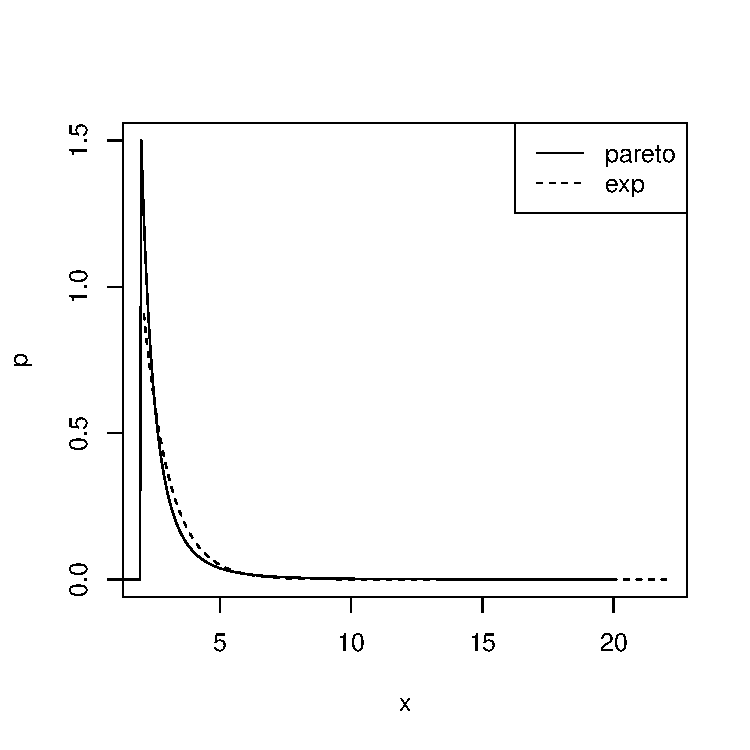
\includegraphics[width=\maxwidth]{figure/r-chunk1-1} 

\end{knitrout}

\subsection{b)}
Firstly, do some basic setting and basic calculation
\begin{knitrout}
\definecolor{shadecolor}{rgb}{0.969, 0.969, 0.969}\color{fgcolor}\begin{kframe}
\begin{alltt}
\hlcom{####basic setting}
\hlstd{beta}\hlkwb{<-}\hlnum{3}\hlstd{;alpha}\hlkwb{<-}\hlnum{2}\hlstd{;lambda}\hlkwb{<-}\hlnum{1}\hlstd{;m}\hlkwb{<-}\hlnum{10000}

\hlcom{####get sample from pareto distribution}
\hlstd{sample_pareto}\hlkwb{<-}\hlkwd{rpareto}\hlstd{(m,}\hlkwc{scale}\hlstd{=alpha,}\hlkwc{shape}\hlstd{=beta)}

\hlcom{####calcualte the expection of x and square of x}
\hlstd{ex_2}\hlkwb{<-}\hlstd{sample_pareto}\hlopt{^}\hlnum{5}\hlopt{*}\hlkwd{exp}\hlstd{(}\hlopt{-}\hlstd{sample_pareto}\hlopt{+}\hlnum{2}\hlstd{)}\hlopt{/}\hlnum{24}
\hlstd{ex_square_2}\hlkwb{<-}\hlstd{sample_pareto}\hlopt{^}\hlnum{6}\hlopt{*}\hlkwd{exp}\hlstd{(}\hlopt{-}\hlstd{sample_pareto}\hlopt{+}\hlnum{2}\hlstd{)}\hlopt{/}\hlnum{24}

\hlcom{####calculate the weight}
\hlstd{weight_2}\hlkwb{<-}\hlstd{sample_pareto}\hlopt{^}\hlnum{4}\hlopt{*}\hlkwd{exp}\hlstd{(}\hlopt{-}\hlstd{sample_pareto}\hlopt{+}\hlnum{2}\hlstd{)}\hlopt{/}\hlnum{24}
\end{alltt}
\end{kframe}
\end{knitrout}

Then show the required expectation and give histogram plots
\begin{knitrout}
\definecolor{shadecolor}{rgb}{0.969, 0.969, 0.969}\color{fgcolor}\begin{kframe}
\begin{alltt}
\hlcom{####calculate the expectation,variance of x and square of x}
\hlkwd{mean}\hlstd{(ex_2);}\hlkwd{mean}\hlstd{(ex_square_2)}
\end{alltt}
\begin{verbatim}
## [1] 2.998046
## [1] 10.05176
\end{verbatim}
\begin{alltt}
\hlkwd{var}\hlstd{(ex_2);}\hlkwd{var}\hlstd{(ex_square_2)}
\end{alltt}
\begin{verbatim}
## [1] 2.406171
## [1] 77.09884
\end{verbatim}
\begin{alltt}
\hlcom{##########plot histogram}
\hlkwd{par}\hlstd{(}\hlkwc{mfrow}\hlstd{=}\hlkwd{c}\hlstd{(}\hlnum{1}\hlstd{,}\hlnum{3}\hlstd{))}
\hlkwd{hist}\hlstd{(ex_2);}\hlkwd{hist}\hlstd{(ex_square_2);}\hlkwd{hist}\hlstd{(weight_2)}
\end{alltt}
\end{kframe}
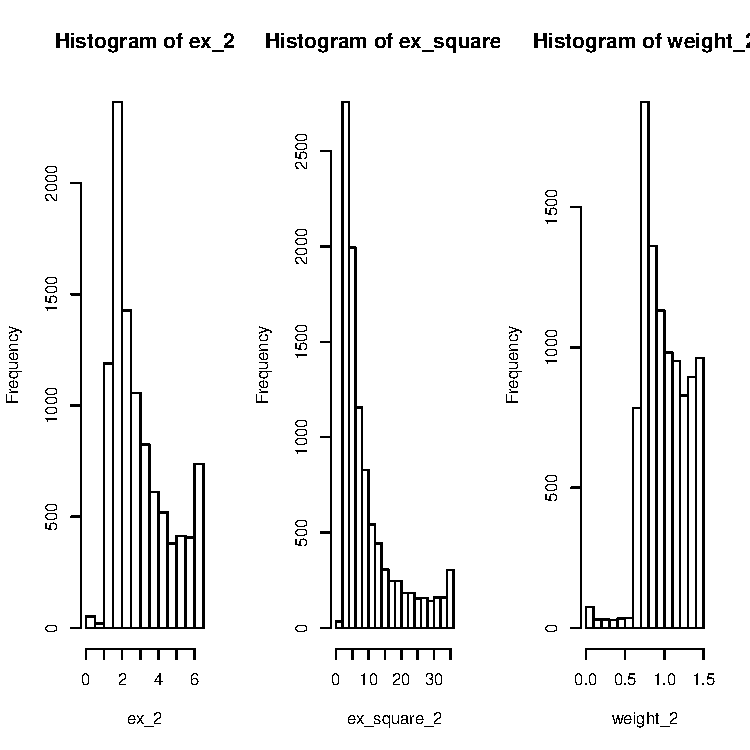
\includegraphics[width=\maxwidth]{figure/r-chunk8-1} 

\end{knitrout}
From the plot, we can find that $h(x)f(x)/g(x)$ and $f(x)/g(x)$ is distributed relatively even. And there is no extreme value. It is beacuse $g(x)$ has heavier tail than $f(x)$.


\subsection{c)}
Do some basic setting and basic calculation the same as section\_b
\begin{knitrout}
\definecolor{shadecolor}{rgb}{0.969, 0.969, 0.969}\color{fgcolor}\begin{kframe}
\begin{alltt}
\hlcom{####sample from exponential distribution}
\hlstd{sample_exp}\hlkwb{<-}\hlkwd{rexp}\hlstd{(m)}\hlopt{+}\hlnum{2}

\hlcom{####calcualte the expection of x and square of x}
\hlstd{ex_3}\hlkwb{<-}\hlnum{24}\hlopt{*}\hlstd{sample_exp}\hlopt{^}\hlstd{(}\hlopt{-}\hlnum{3}\hlstd{)}\hlopt{*}\hlkwd{exp}\hlstd{(sample_exp}\hlopt{-}\hlnum{2}\hlstd{)}
\hlstd{ex_square_3}\hlkwb{<-}\hlnum{24}\hlopt{*}\hlstd{sample_exp}\hlopt{^}\hlstd{(}\hlopt{-}\hlnum{2}\hlstd{)}\hlopt{*}\hlkwd{exp}\hlstd{(sample_exp}\hlopt{-}\hlnum{2}\hlstd{)}

\hlcom{####calculate the weight}
\hlstd{weight_3}\hlkwb{<-}\hlnum{24}\hlopt{*}\hlstd{sample_exp}\hlopt{^}\hlstd{(}\hlopt{-}\hlnum{4}\hlstd{)}\hlopt{*}\hlkwd{exp}\hlstd{(sample_exp}\hlopt{-}\hlnum{2}\hlstd{)}
\end{alltt}
\end{kframe}
\end{knitrout}

show the result.
\begin{knitrout}
\definecolor{shadecolor}{rgb}{0.969, 0.969, 0.969}\color{fgcolor}\begin{kframe}
\begin{alltt}
\hlcom{####calculate the expectation,variance of x and square of x}
\hlkwd{mean}\hlstd{(ex_3);}\hlkwd{mean}\hlstd{(ex_square_3)}
\end{alltt}
\begin{verbatim}
## [1] 2.943074
## [1] 10.48022
\end{verbatim}
\begin{alltt}
\hlkwd{var}\hlstd{(ex_3);}\hlkwd{var}\hlstd{(ex_square_3)}
\end{alltt}
\begin{verbatim}
## [1] 60.22603
## [1] 10295.85
\end{verbatim}
\begin{alltt}
\hlcom{##########plot histogram}
\hlkwd{par}\hlstd{(}\hlkwc{mfrow}\hlstd{=}\hlkwd{c}\hlstd{(}\hlnum{1}\hlstd{,}\hlnum{3}\hlstd{))}
\hlkwd{hist}\hlstd{(ex_3);}\hlkwd{hist}\hlstd{(ex_square_3);}\hlkwd{hist}\hlstd{(weight_3)}
\end{alltt}
\end{kframe}
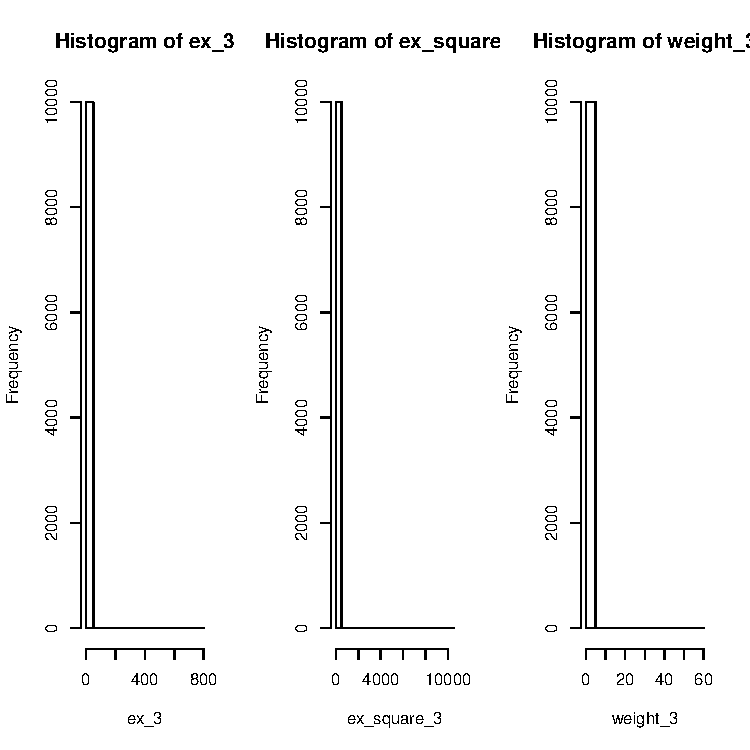
\includegraphics[width=\maxwidth]{figure/r-chunk9-1} 

\end{knitrout}
Each plot shows that there are several extreme values which mean that the variance of estimators would be relatively large. It is beacuse $f(x)$ has heavier tail than $g(x)$.

\section{Question2}
\begin{knitrout}
\definecolor{shadecolor}{rgb}{0.969, 0.969, 0.969}\color{fgcolor}\begin{kframe}
\begin{alltt}
\hlstd{theta} \hlkwb{<-} \hlkwa{function}\hlstd{(}\hlkwc{x1}\hlstd{,}\hlkwc{x2}\hlstd{)} \hlkwd{atan2}\hlstd{(x2, x1)}\hlopt{/}\hlstd{(}\hlnum{2}\hlopt{*}\hlstd{pi)}

\hlstd{f} \hlkwb{<-} \hlkwa{function}\hlstd{(}\hlkwc{x}\hlstd{) \{}
  \hlstd{f1} \hlkwb{<-} \hlnum{10}\hlopt{*}\hlstd{(x[}\hlnum{3}\hlstd{]} \hlopt{-} \hlnum{10}\hlopt{*}\hlkwd{theta}\hlstd{(x[}\hlnum{1}\hlstd{],x[}\hlnum{2}\hlstd{]))}
  \hlstd{f2} \hlkwb{<-} \hlnum{10}\hlopt{*}\hlstd{(}\hlkwd{sqrt}\hlstd{(x[}\hlnum{1}\hlstd{]}\hlopt{^}\hlnum{2} \hlopt{+} \hlstd{x[}\hlnum{2}\hlstd{]}\hlopt{^}\hlnum{2}\hlstd{)} \hlopt{-} \hlnum{1}\hlstd{)}
  \hlstd{f3} \hlkwb{<-} \hlstd{x[}\hlnum{3}\hlstd{]}
  \hlkwd{return}\hlstd{(f1}\hlopt{^}\hlnum{2} \hlopt{+} \hlstd{f2}\hlopt{^}\hlnum{2} \hlopt{+} \hlstd{f3}\hlopt{^}\hlnum{2}\hlstd{)}
\hlstd{\}}
\end{alltt}
\end{kframe}
\end{knitrout}


\begin{knitrout}
\definecolor{shadecolor}{rgb}{0.969, 0.969, 0.969}\color{fgcolor}\begin{kframe}
\begin{alltt}
\hlcom{####fix x3 and calculate the value of f(c(x1,x2,0))}

\hlcom{###set x from -5 to 5 and get 201 values}
\hlstd{x1}\hlkwb{<-}\hlkwd{seq}\hlstd{(}\hlopt{-}\hlnum{5}\hlstd{,}\hlnum{5}\hlstd{,}\hlnum{0.05}\hlstd{)}
\hlstd{x2}\hlkwb{<-}\hlkwd{seq}\hlstd{(}\hlopt{-}\hlnum{5}\hlstd{,}\hlnum{5}\hlstd{,}\hlnum{0.05}\hlstd{)}
\hlstd{x3}\hlkwb{<-}\hlkwd{seq}\hlstd{(}\hlopt{-}\hlnum{5}\hlstd{,}\hlnum{5}\hlstd{,}\hlnum{0.05}\hlstd{)}
\hlstd{f_value12}\hlkwb{<-}\hlkwd{matrix}\hlstd{(}\hlkwc{nrow}\hlstd{=}\hlnum{201}\hlstd{,}\hlkwc{ncol}\hlstd{=}\hlnum{201}\hlstd{)}
\hlkwa{for}\hlstd{(i} \hlkwa{in} \hlnum{1}\hlopt{:}\hlnum{201}\hlstd{)\{}
  \hlkwa{for}\hlstd{(j} \hlkwa{in} \hlnum{1}\hlopt{:}\hlnum{201}\hlstd{)\{}
    \hlstd{f_value12[i,j]}\hlkwb{<-}\hlkwd{f}\hlstd{(}\hlkwd{c}\hlstd{(x1[i],x2[j],}\hlnum{0}\hlstd{))}
  \hlstd{\}}
\hlstd{\}}
\hlcom{####fix x2 as 0}
\hlstd{f_value13}\hlkwb{<-}\hlkwd{matrix}\hlstd{(}\hlkwc{nrow}\hlstd{=}\hlnum{201}\hlstd{,}\hlkwc{ncol}\hlstd{=}\hlnum{201}\hlstd{)}
\hlkwa{for}\hlstd{(i} \hlkwa{in} \hlnum{1}\hlopt{:}\hlnum{201}\hlstd{)\{}
  \hlkwa{for}\hlstd{(j} \hlkwa{in} \hlnum{1}\hlopt{:}\hlnum{201}\hlstd{)\{}
    \hlstd{f_value13[i,j]}\hlkwb{<-}\hlkwd{f}\hlstd{(}\hlkwd{c}\hlstd{(x1[i],}\hlnum{0}\hlstd{,x3[j]))}
  \hlstd{\}}
\hlstd{\}}

\hlcom{####fix x1 as 1}
\hlstd{f_value23}\hlkwb{<-}\hlkwd{matrix}\hlstd{(}\hlkwc{nrow}\hlstd{=}\hlnum{201}\hlstd{,}\hlkwc{ncol}\hlstd{=}\hlnum{201}\hlstd{)}
\hlkwa{for}\hlstd{(i} \hlkwa{in} \hlnum{1}\hlopt{:}\hlnum{201}\hlstd{)\{}
  \hlkwa{for}\hlstd{(j} \hlkwa{in} \hlnum{1}\hlopt{:}\hlnum{201}\hlstd{)\{}
    \hlstd{f_value23[i,j]}\hlkwb{<-}\hlkwd{f}\hlstd{(}\hlkwd{c}\hlstd{(}\hlnum{1}\hlstd{,x2[i],x3[j]))}
  \hlstd{\}}
\hlstd{\}}
\end{alltt}
\end{kframe}
\end{knitrout}


\begin{knitrout}
\definecolor{shadecolor}{rgb}{0.969, 0.969, 0.969}\color{fgcolor}\begin{kframe}
\begin{alltt}
\hlcom{########compare the plot}
\hlkwd{par}\hlstd{(}\hlkwc{mfrow}\hlstd{=}\hlkwd{c}\hlstd{(}\hlnum{1}\hlstd{,}\hlnum{3}\hlstd{))}
\hlkwd{image}\hlstd{(x1,x2,f_value12)}
\hlkwd{contour}\hlstd{(x1,x2,f_value12,}\hlkwc{add}\hlstd{=}\hlnum{TRUE}\hlstd{,}\hlkwc{drawlabels} \hlstd{=} \hlnum{FALSE}\hlstd{)}
\hlkwd{image}\hlstd{(x1,x3,f_value13)}
\hlkwd{contour}\hlstd{(x1,x3,f_value13,}\hlkwc{add}\hlstd{=}\hlnum{TRUE}\hlstd{,}\hlkwc{drawlabels} \hlstd{=} \hlnum{FALSE}\hlstd{)}
\hlkwd{image}\hlstd{(x2,x3,f_value23)}
\hlkwd{contour}\hlstd{(x2,x3,f_value23,}\hlkwc{add}\hlstd{=}\hlnum{TRUE}\hlstd{,}\hlkwc{drawlabels} \hlstd{=} \hlnum{FALSE}\hlstd{)}
\end{alltt}
\end{kframe}
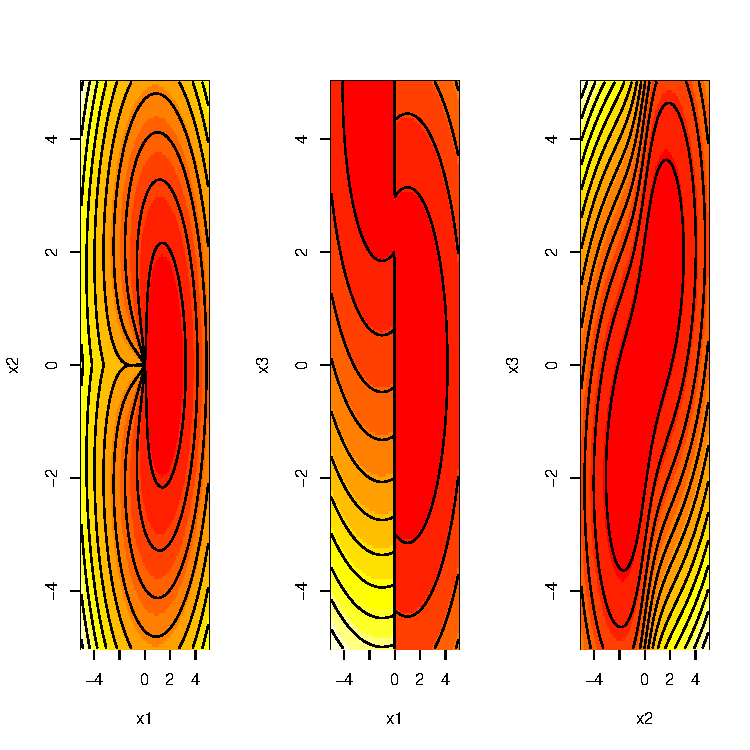
\includegraphics[width=\maxwidth]{figure/r-chunk6-1} 

\end{knitrout}

\begin{knitrout}
\definecolor{shadecolor}{rgb}{0.969, 0.969, 0.969}\color{fgcolor}\begin{kframe}
\begin{alltt}
\hlcom{############calculate the optimum of f function}
\hlstd{start}\hlkwb{<-}\hlkwd{c}\hlstd{(}\hlnum{100}\hlstd{,}\hlopt{-}\hlnum{10}\hlstd{,}\hlopt{-}\hlnum{10}\hlstd{)}
\hlstd{op}\hlkwb{<-}\hlkwd{optim}\hlstd{(}\hlkwc{par}\hlstd{=start,}\hlkwc{fn}\hlstd{=f)}
\hlstd{nl}\hlkwb{<-}\hlkwd{nlm}\hlstd{(}\hlkwc{f}\hlstd{=f,}\hlkwc{p}\hlstd{=start)}
\hlstd{op}\hlopt{$}\hlstd{par;op}\hlopt{$}\hlstd{value;nl}\hlopt{$}\hlstd{estimate;nl}\hlopt{$}\hlstd{minimum}
\end{alltt}
\begin{verbatim}
## [1]  1.000634580 -0.001903183 -0.001726437
## [1] 0.0002126484
## [1]  1.000000e+00 -2.142877e-10  3.478953e-10
## [1] 7.203601e-17
\end{verbatim}
\begin{alltt}
\hlstd{start}\hlkwb{<-}\hlkwd{c}\hlstd{(}\hlnum{20}\hlstd{,}\hlnum{100}\hlstd{,}\hlnum{1}\hlstd{)}
\hlstd{op}\hlkwb{<-}\hlkwd{optim}\hlstd{(}\hlkwc{par}\hlstd{=start,}\hlkwc{fn}\hlstd{=f)}
\hlstd{op}\hlopt{$}\hlstd{par;op}\hlopt{$}\hlstd{value}
\end{alltt}
\begin{verbatim}
## [1]  0.9884603 -0.1617380 -0.2637370
## [1] 0.07295685
\end{verbatim}
\begin{alltt}
\hlstd{start}\hlkwb{<-}\hlkwd{c}\hlstd{(}\hlnum{1}\hlstd{,}\hlnum{1}\hlstd{,}\hlnum{1}\hlstd{)}
\hlstd{op}\hlkwb{<-}\hlkwd{optim}\hlstd{(}\hlkwc{par}\hlstd{=start,}\hlkwc{fn}\hlstd{=f)}
\hlstd{op}\hlopt{$}\hlstd{par;op}\hlopt{$}\hlstd{value}
\end{alltt}
\begin{verbatim}
## [1]  0.9999779414 -0.0001349269 -0.0001927127
## [1] 1.343098e-07
\end{verbatim}
\begin{alltt}
\hlstd{start}\hlkwb{<-}\hlkwd{c}\hlstd{(}\hlnum{1}\hlstd{,}\hlnum{0}\hlstd{,}\hlnum{0}\hlstd{)}
\hlstd{op}\hlkwb{<-}\hlkwd{optim}\hlstd{(}\hlkwc{par}\hlstd{=start,}\hlkwc{fn}\hlstd{=f)}
\hlstd{nl}\hlkwb{<-}\hlkwd{nlm}\hlstd{(}\hlkwc{f}\hlstd{=f,}\hlkwc{p}\hlstd{=start)}
\hlstd{op}\hlopt{$}\hlstd{par;op}\hlopt{$}\hlstd{value;nl}\hlopt{$}\hlstd{estimate;nl}\hlopt{$}\hlstd{minimum}
\end{alltt}
\begin{verbatim}
## [1] 1 0 0
## [1] 0
## [1] 1 0 0
## [1] 0
\end{verbatim}
\end{kframe}
\end{knitrout}
From the result, we find all optimum is around 0, and the coordinates are around $(1,0,0)$. And when we set the start as $(1,0,0)$, the optimum equals to 0. And explore the function f, it returns the sum of three squares, so 0 is the global optimum. And I find nlm get better results.


\section{Question3}
\subsection{a)}
Algorithm:\\

step1: first write the $Q(\theta|\theta_t)$
\begin{align*}
 Q(\theta|\theta_t)&=E(log L(\theta|Y)|x,\theta_t)\\
                   &=-\frac{n}{2}log(2\pi\sigma^2)-\frac{1}{2\sigma^2}\sum_{i=c+1}^n(y_i-\beta_0-\beta_1x_i)^2-\frac{1}{2\sigma^2}E([\sum_{i=1}^cZ_i^2-2(\beta_0+\beta_1x_i)\sum_{i=1}^cZ_i+\sum_{i=1}^c(\beta_0+\beta_1x_i)^2]|(\theta_t,x))
  \end{align*}
  
step2: we want to maximize the $Q(\theta|\theta_t)$, which means minimizes $-Q(\theta|\theta_t)$;let $A_i=E(Z_i^2|(\theta_t,x)),B_i=E(Z_i|\theta_t,x)$, A and B are both constants given $\theta_t,x$. 
\begin{align*}
 -Q(\theta|\theta_t)&=-E(log L(\theta|Y)|x,\theta_t)\\
                    &=\frac{1}{2\sigma^2}(n\sigma^2log(2\pi\sigma^2)+\sum_{i=c+1}^n(y_i-\beta_0-\beta_1x_i)^2+[\sum_{i=1}^cA_i-2\sum_{i=1}^c(\beta_0+\beta_1x_i)B_i+\sum_{i=1}^c(\beta_0+\beta_1x_i)^2])\\
                    &=\frac{1}{2\sigma^2}(n\sigma^2log(2\pi\sigma^2)+\sum_{i=c+1}^n(y_i-\beta_0-\beta_1x_i)^2+\sum_{i=1}^c(B_i-\beta_0-\beta_1x_i)^2-\sum_{i=1}^{c}B_i^2+\sum_{i=1}^{c}A_i)
  \end{align*}
  
step3:As A,B,c are all constants, if we want to minimize $-Q(\theta|\theta_t)$, we first should minimize $\sum_{i=c+1}^n(y_i-\beta_0-\beta_1x_i)^2+\sum_{i=1}^c(B_i-\beta_0-\beta_1x_i)^2$. It is exactly the RSS of regression of $(y,x)$, where the first c elements in $y_i$ equals to $B_i$, and the latter are $y_i$. In this way, we can get the $\hat{\beta_0},\hat{\beta_1}$ from linear regression\\

After get the RSS, we then do derivation to $\sigma^2$ and get $\hat{\sigma}^2$\\

step4:let $\theta_{t+1}=(\hat{\beta_0},\hat{\beta_1},\hat{\sigma}^2)$ and return to step2, do iteration until $||\theta_t-\theta_{t+1}||<m$, m=0.00001 is a small constant we set to stop the iteration, or if the iteration times over 1000, I also stop the loop.


\subsection{b)}
As we only have n-c complete data $(x,y)$, use lm function to $(y~x)$ and get the coefficients of the linear regression. Then I take $\beta_0$ as the first coefficient and take $\beta_1$ as the second coefficient, also take $\sigma_0^2$ as $RSS/n$.

\subsection{c)}
\begin{knitrout}
\definecolor{shadecolor}{rgb}{0.969, 0.969, 0.969}\color{fgcolor}\begin{kframe}
\begin{alltt}
\hlcom{######## write ez function to get the expectation of Z and Z^2;}
\hlcom{######## which in my algorithm in (a) equals to Bi and Ai}
\hlstd{ez}\hlkwb{<-}\hlkwa{function}\hlstd{(}\hlkwc{mu}\hlstd{,}\hlkwc{sigma}\hlstd{,}\hlkwc{k}\hlstd{)\{}
  \hlstd{result}\hlkwb{<-}\hlkwd{c}\hlstd{()}

  \hlcom{###calculate the Ez and Ez^2}
  \hlstd{k_star}\hlkwb{<-}\hlstd{(k}\hlopt{-}\hlstd{mu)}\hlopt{/}\hlstd{sigma}
  \hlstd{r_kstar}\hlkwb{<-}\hlkwd{dnorm}\hlstd{(k_star)}\hlopt{/}\hlstd{(}\hlnum{1}\hlopt{-}\hlkwd{pnorm}\hlstd{(k_star))}

  \hlcom{###store the value in a vector}
  \hlstd{result[}\hlnum{1}\hlstd{]}\hlkwb{<-}\hlstd{mu}\hlopt{+}\hlstd{sigma}\hlopt{*}\hlstd{r_kstar}
  \hlstd{result[}\hlnum{2}\hlstd{]}\hlkwb{<-}\hlstd{result[}\hlnum{1}\hlstd{]}\hlopt{^}\hlnum{2}\hlopt{+}\hlstd{sigma}\hlopt{^}\hlnum{2}\hlopt{*}\hlstd{(}\hlnum{1}\hlopt{+}\hlstd{k_star}\hlopt{*}\hlstd{r_kstar}\hlopt{-}\hlstd{r_kstar}\hlopt{^}\hlnum{2}\hlstd{)}
  \hlkwd{return}\hlstd{(result)}
\hlstd{\}}

\hlcom{###write the function to get censored y according to the given proportion}
\hlstd{censored_y}\hlkwb{<-}\hlkwa{function}\hlstd{(}\hlkwc{x}\hlstd{,}\hlkwc{y}\hlstd{,}\hlkwc{proportion}\hlstd{,}\hlkwc{beta}\hlstd{)\{}
  \hlstd{b}\hlkwb{<-}\hlkwd{rep}\hlstd{(}\hlnum{0}\hlstd{,}\hlnum{100}\hlstd{);a}\hlkwb{<-}\hlkwd{rep}\hlstd{(}\hlnum{0}\hlstd{,}\hlnum{100}\hlstd{)}
  \hlstd{tau}\hlkwb{<-}\hlkwd{sort}\hlstd{(yComplete)[n}\hlopt{-}\hlstd{n}\hlopt{*}\hlstd{proportion}\hlopt{+}\hlnum{1}\hlstd{]}

  \hlcom{###find the y needed to be censored and then calaulate the corresponding Bi and Ai}
  \hlkwa{for}\hlstd{(i} \hlkwa{in} \hlnum{1}\hlopt{:}\hlstd{n)\{}
    \hlkwa{if} \hlstd{(y[i]}\hlopt{>=}\hlstd{tau) \{}
      \hlstd{y[i]}\hlkwb{<-}\hlkwd{ez}\hlstd{(beta[}\hlnum{1}\hlstd{]}\hlopt{+}\hlstd{beta[}\hlnum{2}\hlstd{]}\hlopt{*}\hlstd{x[i],}\hlkwd{sqrt}\hlstd{(beta[}\hlnum{3}\hlstd{]),tau)[}\hlnum{1}\hlstd{]}
      \hlstd{b[i]}\hlkwb{<-}\hlstd{y[i]}
      \hlstd{a[i]}\hlkwb{<-}\hlkwd{ez}\hlstd{(beta[}\hlnum{1}\hlstd{]}\hlopt{+}\hlstd{beta[}\hlnum{2}\hlstd{]}\hlopt{*}\hlstd{x[i],}\hlkwd{sqrt}\hlstd{(beta[}\hlnum{3}\hlstd{]),tau)[}\hlnum{2}\hlstd{]}
    \hlstd{\}}
  \hlstd{\}}
  \hlcom{###store the result in a matrix}
  \hlstd{data}\hlkwb{<-}\hlkwd{cbind}\hlstd{(y,a,b)}
  \hlkwd{return}\hlstd{(data)}
\hlstd{\}}

\hlcom{####write the final function to get estimated theta}
\hlstd{em}\hlkwb{<-}\hlkwa{function}\hlstd{(}\hlkwc{proportion}\hlstd{)\{}

  \hlcom{###get x and y}
  \hlkwd{set.seed}\hlstd{(}\hlnum{1}\hlstd{)}
  \hlstd{n} \hlkwb{<-} \hlnum{100}\hlstd{; beta0} \hlkwb{<-} \hlnum{1}\hlstd{; beta1} \hlkwb{<-} \hlnum{2}\hlstd{; sigma2} \hlkwb{<-} \hlnum{6}
  \hlstd{x} \hlkwb{<-} \hlkwd{runif}\hlstd{(n)}
  \hlstd{b}\hlkwb{<-}\hlkwd{rep}\hlstd{(}\hlnum{0}\hlstd{,}\hlnum{100}\hlstd{);a}\hlkwb{<-}\hlkwd{rep}\hlstd{(}\hlnum{0}\hlstd{,}\hlnum{100}\hlstd{)}
  \hlstd{yComplete} \hlkwb{<-} \hlkwd{rnorm}\hlstd{(n, beta0} \hlopt{+} \hlstd{beta1}\hlopt{*}\hlstd{x,} \hlkwd{sqrt}\hlstd{(sigma2))}

  \hlcom{###initiate some settings}
  \hlstd{itera}\hlkwb{<-}\hlnum{0}\hlstd{;beta_0}\hlkwb{<-}\hlkwd{c}\hlstd{();beta_1}\hlkwb{<-}\hlkwd{c}\hlstd{();error}\hlkwb{<-}\hlnum{100}

  \hlcom{########to calculate the initial beta, first calculate the complete x and y}
  \hlstd{tau}\hlkwb{<-}\hlkwd{sort}\hlstd{(yComplete)[n}\hlopt{-}\hlstd{n}\hlopt{*}\hlstd{proportion}\hlopt{+}\hlnum{1}\hlstd{]}
  \hlstd{y0}\hlkwb{<-}\hlkwd{c}\hlstd{();x0}\hlkwb{<-}\hlkwd{c}\hlstd{()}
  \hlstd{y0}\hlkwb{<-}\hlstd{yComplete[}\hlkwd{which}\hlstd{(yComplete}\hlopt{<}\hlstd{tau)]}
  \hlstd{x0}\hlkwb{<-}\hlstd{x[}\hlkwd{which}\hlstd{(yComplete}\hlopt{<}\hlstd{tau)]}

  \hlcom{######calculate the beta_0}
  \hlstd{lm0}\hlkwb{<-}\hlkwd{lm}\hlstd{(y0}\hlopt{~}\hlstd{x0)}
  \hlstd{beta_0[}\hlnum{1}\hlstd{]}\hlkwb{<-}\hlkwd{summary}\hlstd{(lm0)}\hlopt{$}\hlstd{coef[}\hlnum{1}\hlstd{]}
  \hlstd{beta_0[}\hlnum{2}\hlstd{]}\hlkwb{<-}\hlkwd{summary}\hlstd{(lm0)}\hlopt{$}\hlstd{coef[}\hlnum{2}\hlstd{]}
  \hlstd{beta_0[}\hlnum{3}\hlstd{]}\hlkwb{<-}\hlkwd{sum}\hlstd{(lm0}\hlopt{$}\hlstd{residuals}\hlopt{^}\hlnum{2}\hlstd{)}\hlopt{/}\hlkwd{length}\hlstd{(y0)}

  \hlcom{###do iteration until the number of iteration is over 1000 times or the error is smaller than 0.00001}
  \hlkwa{while}\hlstd{(error}\hlopt{>=}\hlnum{0.00001}\hlopt{&}\hlstd{itera}\hlopt{<=}\hlnum{1000}\hlstd{)\{}
    \hlstd{itera}\hlkwb{<-}\hlstd{itera}\hlopt{+}\hlnum{1}
    \hlstd{yab}\hlkwb{<-}\hlkwd{censored_y}\hlstd{(x,yComplete,proportion,beta_0)}
    \hlstd{y}\hlkwb{<-}\hlstd{yab[,}\hlnum{1}\hlstd{]}
    \hlstd{a}\hlkwb{<-}\hlstd{yab[,}\hlnum{2}\hlstd{]}
    \hlstd{b}\hlkwb{<-}\hlstd{yab[,}\hlnum{3}\hlstd{]}
    \hlstd{lm}\hlkwb{<-}\hlkwd{lm}\hlstd{(y}\hlopt{~}\hlstd{x)}

    \hlcom{###get a new beta}
    \hlstd{beta_1[}\hlnum{1}\hlstd{]}\hlkwb{<-}\hlkwd{summary}\hlstd{(lm)}\hlopt{$}\hlstd{coef[}\hlnum{1}\hlstd{]}
    \hlstd{beta_1[}\hlnum{2}\hlstd{]}\hlkwb{<-}\hlkwd{summary}\hlstd{(lm)}\hlopt{$}\hlstd{coef[}\hlnum{2}\hlstd{]}
    \hlstd{beta_1[}\hlnum{3}\hlstd{]}\hlkwb{<-}\hlstd{(}\hlkwd{sum}\hlstd{(lm}\hlopt{$}\hlstd{residuals}\hlopt{^}\hlnum{2}\hlstd{)}\hlopt{-}\hlkwd{crossprod}\hlstd{(b)}\hlopt{+}\hlkwd{sum}\hlstd{(a))}\hlopt{/}\hlstd{n}

    \hlcom{####calculate the error between new beta and old beta}
    \hlstd{error}\hlkwb{<-}\hlkwd{crossprod}\hlstd{(beta_0}\hlopt{-}\hlstd{beta_1)}
    \hlstd{beta_0}\hlkwb{<-}\hlstd{beta_1}
  \hlstd{\}}
  \hlkwd{return}\hlstd{(}\hlkwd{c}\hlstd{(beta_0,error,itera))}
\hlstd{\}}
\hlkwd{em}\hlstd{(}\hlnum{0.2}\hlstd{);}\hlkwd{em}\hlstd{(}\hlnum{0.8}\hlstd{)}
\end{alltt}
\begin{verbatim}
## [1] 4.580421e-01 2.832377e+00 4.654111e+00 2.669040e-06 7.000000e+00
## [1] 3.290495e-01 2.899787e+00 3.899489e+00 9.252086e-06 5.800000e+01
\end{verbatim}
\end{kframe}
\end{knitrout}
The first three values are estimated parameters. From the result, we can find that the estimated parameters converge to the true value. It is also obvious that when we lose 80 percent data, the precise of estimation decreases.

\subsection{d)}
\begin{knitrout}
\definecolor{shadecolor}{rgb}{0.969, 0.969, 0.969}\color{fgcolor}\begin{kframe}
\begin{alltt}
\hlcom{###function to calculate the log likelihood value}
\hlstd{f}\hlkwb{<-}\hlkwa{function}\hlstd{(}\hlkwc{input}\hlstd{,}\hlkwc{proportion}\hlstd{=}\hlnum{0.2}\hlstd{)\{}
  \hlstd{beta00}\hlkwb{<-}\hlstd{input[}\hlnum{1}\hlstd{];beta01}\hlkwb{<-}\hlstd{input[}\hlnum{2}\hlstd{];sigma_square}\hlkwb{<-}\hlstd{input[}\hlnum{3}\hlstd{]}

  \hlkwd{set.seed}\hlstd{(}\hlnum{1}\hlstd{)}
  \hlstd{n} \hlkwb{<-} \hlnum{100}\hlstd{; beta0} \hlkwb{<-} \hlnum{1}\hlstd{; beta1} \hlkwb{<-} \hlnum{2}\hlstd{; sigma2} \hlkwb{<-} \hlnum{6}
  \hlstd{x} \hlkwb{<-} \hlkwd{runif}\hlstd{(n); yComplete} \hlkwb{<-} \hlkwd{rnorm}\hlstd{(n, beta0} \hlopt{+} \hlstd{beta1}\hlopt{*}\hlstd{x,} \hlkwd{sqrt}\hlstd{(sigma2))}

  \hlcom{###get two parts of data(x,y)}
  \hlstd{tau}\hlkwb{<-}\hlkwd{sort}\hlstd{(yComplete)[n}\hlopt{-}\hlstd{n}\hlopt{*}\hlstd{proportion}\hlopt{+}\hlnum{1}\hlstd{]}
  \hlstd{y_censored}\hlkwb{<-}\hlstd{yComplete[}\hlkwd{which}\hlstd{(yComplete}\hlopt{>=}\hlstd{tau)]}
  \hlstd{x_censored}\hlkwb{<-}\hlstd{x[}\hlkwd{which}\hlstd{(yComplete}\hlopt{>=}\hlstd{tau)]}
  \hlstd{y_complete}\hlkwb{<-}\hlstd{yComplete[}\hlkwd{which}\hlstd{(yComplete}\hlopt{<}\hlstd{tau)]}
  \hlstd{x_complete}\hlkwb{<-}\hlstd{x[}\hlkwd{which}\hlstd{(yComplete}\hlopt{<}\hlstd{tau)]}

  \hlcom{###calculate the log likelihood value of censored data and complete data}
  \hlstd{l_censored}\hlkwb{<-}\hlkwd{sum}\hlstd{(}\hlkwd{log}\hlstd{(}\hlnum{1}\hlopt{-}\hlkwd{pnorm}\hlstd{((tau}\hlopt{-}\hlstd{beta00}\hlopt{-}\hlstd{beta01}\hlopt{*}\hlstd{x_censored)}\hlopt{/}\hlkwd{sqrt}\hlstd{(sigma_square))))}
  \hlstd{l_complete}\hlkwb{=}\hlopt{-}\hlstd{n}\hlopt{*}\hlstd{(}\hlnum{1}\hlopt{-}\hlstd{proportion)}\hlopt{/}\hlnum{2}\hlopt{*}\hlkwd{log}\hlstd{(}\hlnum{2}\hlopt{*}\hlstd{pi}\hlopt{*}\hlstd{sigma_square)}\hlopt{-}\hlnum{1}\hlopt{/}\hlstd{(}\hlnum{2}\hlopt{*}\hlstd{sigma_square)}\hlopt{*}
  \hlkwd{crossprod}\hlstd{(y_complete}\hlopt{-}\hlstd{beta00}\hlopt{-}\hlstd{beta01}\hlopt{*}\hlstd{x_complete)}

  \hlcom{###return the negative of sum of two log likelihood value}
  \hlkwd{return}\hlstd{(}\hlopt{-}\hlstd{(l_censored}\hlopt{+}\hlstd{l_complete))}

\hlstd{\}}

\hlcom{###get the result and compare with my EM algorithm}
\hlstd{op}\hlkwb{<-}\hlkwd{optim}\hlstd{(}\hlkwc{par}\hlstd{=}\hlkwd{c}\hlstd{(}\hlnum{1}\hlstd{,}\hlnum{1}\hlstd{,}\hlnum{1}\hlstd{),}\hlkwc{fn}\hlstd{=f,}\hlkwc{lower}\hlstd{=}\hlkwd{c}\hlstd{(}\hlnum{0}\hlstd{,}\hlnum{0}\hlstd{,}\hlnum{0}\hlstd{),}\hlkwc{method} \hlstd{=} \hlstr{'BFGS'}\hlstd{)}
\hlstd{op}\hlopt{$}\hlstd{par;op}\hlopt{$}\hlstd{counts}
\end{alltt}
\begin{verbatim}
## [1] 0.4580453 2.8325579 4.6548216
## function gradient 
##       15       15
\end{verbatim}
\begin{alltt}
\hlkwd{em}\hlstd{(}\hlnum{0.2}\hlstd{)[}\hlnum{1}\hlopt{:}\hlnum{3}\hlstd{];}\hlkwd{em}\hlstd{(}\hlnum{0.2}\hlstd{)[}\hlnum{5}\hlstd{]}
\end{alltt}
\begin{verbatim}
## [1] 0.4580421 2.8323768 4.6541108
## [1] 7
\end{verbatim}
\begin{alltt}
\hlcom{###########################################################}
\hlcom{####try the situation of proportion equals to 0.8}
\hlstd{f}\hlkwb{<-}\hlkwa{function}\hlstd{(}\hlkwc{input}\hlstd{,}\hlkwc{proportion}\hlstd{=}\hlnum{0.8}\hlstd{)\{}
  \hlstd{beta00}\hlkwb{<-}\hlstd{input[}\hlnum{1}\hlstd{];beta01}\hlkwb{<-}\hlstd{input[}\hlnum{2}\hlstd{];sigma_square}\hlkwb{<-}\hlstd{input[}\hlnum{3}\hlstd{]}

  \hlkwd{set.seed}\hlstd{(}\hlnum{1}\hlstd{)}
  \hlstd{n} \hlkwb{<-} \hlnum{100}\hlstd{; beta0} \hlkwb{<-} \hlnum{1}\hlstd{; beta1} \hlkwb{<-} \hlnum{2}\hlstd{; sigma2} \hlkwb{<-} \hlnum{6}
  \hlstd{x} \hlkwb{<-} \hlkwd{runif}\hlstd{(n); yComplete} \hlkwb{<-} \hlkwd{rnorm}\hlstd{(n, beta0} \hlopt{+} \hlstd{beta1}\hlopt{*}\hlstd{x,} \hlkwd{sqrt}\hlstd{(sigma2))}

  \hlcom{###get two parts of data(x,y)}
  \hlstd{tau}\hlkwb{<-}\hlkwd{sort}\hlstd{(yComplete)[n}\hlopt{-}\hlstd{n}\hlopt{*}\hlstd{proportion}\hlopt{+}\hlnum{1}\hlstd{]}
  \hlstd{y_censored}\hlkwb{<-}\hlstd{yComplete[}\hlkwd{which}\hlstd{(yComplete}\hlopt{>=}\hlstd{tau)]}
  \hlstd{x_censored}\hlkwb{<-}\hlstd{x[}\hlkwd{which}\hlstd{(yComplete}\hlopt{>=}\hlstd{tau)]}
  \hlstd{y_complete}\hlkwb{<-}\hlstd{yComplete[}\hlkwd{which}\hlstd{(yComplete}\hlopt{<}\hlstd{tau)]}
  \hlstd{x_complete}\hlkwb{<-}\hlstd{x[}\hlkwd{which}\hlstd{(yComplete}\hlopt{<}\hlstd{tau)]}

  \hlcom{###calculate the log likelihood value of censored data and complete data}
  \hlstd{l_censored}\hlkwb{<-}\hlkwd{sum}\hlstd{(}\hlkwd{log}\hlstd{(}\hlnum{1}\hlopt{-}\hlkwd{pnorm}\hlstd{((tau}\hlopt{-}\hlstd{beta00}\hlopt{-}\hlstd{beta01}\hlopt{*}\hlstd{x_censored)}\hlopt{/}\hlkwd{sqrt}\hlstd{(sigma_square))))}
  \hlstd{l_complete}\hlkwb{=}\hlopt{-}\hlstd{n}\hlopt{*}\hlstd{(}\hlnum{1}\hlopt{-}\hlstd{proportion)}\hlopt{/}\hlnum{2}\hlopt{*}\hlkwd{log}\hlstd{(}\hlnum{2}\hlopt{*}\hlstd{pi}\hlopt{*}\hlstd{sigma_square)}\hlopt{-}\hlnum{1}\hlopt{/}\hlstd{(}\hlnum{2}\hlopt{*}\hlstd{sigma_square)}\hlopt{*}
  \hlkwd{crossprod}\hlstd{(y_complete}\hlopt{-}\hlstd{beta00}\hlopt{-}\hlstd{beta01}\hlopt{*}\hlstd{x_complete)}

  \hlcom{###return the negative of sum of two log likelihood value}
  \hlkwd{return}\hlstd{(}\hlopt{-}\hlstd{(l_censored}\hlopt{+}\hlstd{l_complete))}

\hlstd{\}}

\hlcom{###get the result and compare with my EM algorithm}
\hlstd{op}\hlkwb{<-}\hlkwd{optim}\hlstd{(}\hlkwc{par}\hlstd{=}\hlkwd{c}\hlstd{(}\hlnum{1}\hlstd{,}\hlnum{1}\hlstd{,}\hlnum{1}\hlstd{),}\hlkwc{fn}\hlstd{=f,}\hlkwc{lower}\hlstd{=}\hlkwd{c}\hlstd{(}\hlnum{0}\hlstd{,}\hlnum{0}\hlstd{,}\hlnum{0}\hlstd{),}\hlkwc{method} \hlstd{=} \hlstr{'BFGS'}\hlstd{)}
\hlstd{op}\hlopt{$}\hlstd{par;op}\hlopt{$}\hlstd{counts}
\end{alltt}
\begin{verbatim}
## [1] 0.3332969 2.9135182 3.9322390
## function gradient 
##       14       14
\end{verbatim}
\begin{alltt}
\hlkwd{em}\hlstd{(}\hlnum{0.8}\hlstd{)[}\hlnum{1}\hlopt{:}\hlnum{3}\hlstd{];}\hlkwd{em}\hlstd{(}\hlnum{0.8}\hlstd{)[}\hlnum{5}\hlstd{]}
\end{alltt}
\begin{verbatim}
## [1] 0.3290495 2.8997866 3.8994888
## [1] 58
\end{verbatim}
\end{kframe}
\end{knitrout}
I set proportion$=0.2,0.8$ and compare two algorithms. We can see that the results are both similar. But when proportion equals to 0.2, my EM algorithm costs fewer iterations while when proportion equals to 0.8, my EM algorithm costs much more iterations.  

\end{document}
